% ── Section 4: Chlorophyll case-study results ─────────────
\section{Chlorophyll Case Study: Benchmark Results}
\label{sec:chl_results}

This section reports the chlorophyll reconstruction results on the daily
$\log_{10}(\texttt{chl\_mean})$ target. The headline method comparison uses a strict
artificial-gap support: 449 gaps, 3999 hidden target days, and
$L\in\{1,3,7,14,30\}$~days. Diagnostics that use a different support, such as TS-ICL calibration or covariate-placebo checks, are labelled separately.

\subsection{Artificial-gap benchmark}
\label{sec:chl_benchmark}

Figure~\ref{fig:chl_benchmark_matched} gives the main chlorophyll benchmark. Linear interpolation
is a strong reference: its pooled MAE is 0.239 in $\log_{10}$ units and its error remains close
to the best target-aware methods at short gaps. The strongest external-only tabular model (ExtraTrees) is not competitive. It is worse than
interpolation at every plotted gap length, showing that the tested external predictors alone do
not reconstruct the nearshore chlorophyll target reliably.

The target-only Gaussian process and the gap-edge residual model improve on interpolation in
different regimes. The Gaussian process is strongest at the shortest gaps, where local target
continuity carries most of the recoverable signal, while the gap-edge residual model is worse than
interpolation at $L=1$ and $L=3$, but becomes useful from $L=7$ onward. 

The lowest error at every plotted gap length is obtained by TS-ICL with the satellite-proxy
covariate. The advantage is largest against the
external-only tabular model and smaller, but still resolved, against the target-aware
comparators. Thus, on the chlorophyll benchmark, TS-ICL satellite-proxy is the strongest
single method. This is notable because TS-ICL is used zero-shot: its parameters are not fine-tuned on Tongoy data, although the visible target and covariate context are provided at inference.

\begin{figure}[htbp]
  \centering
  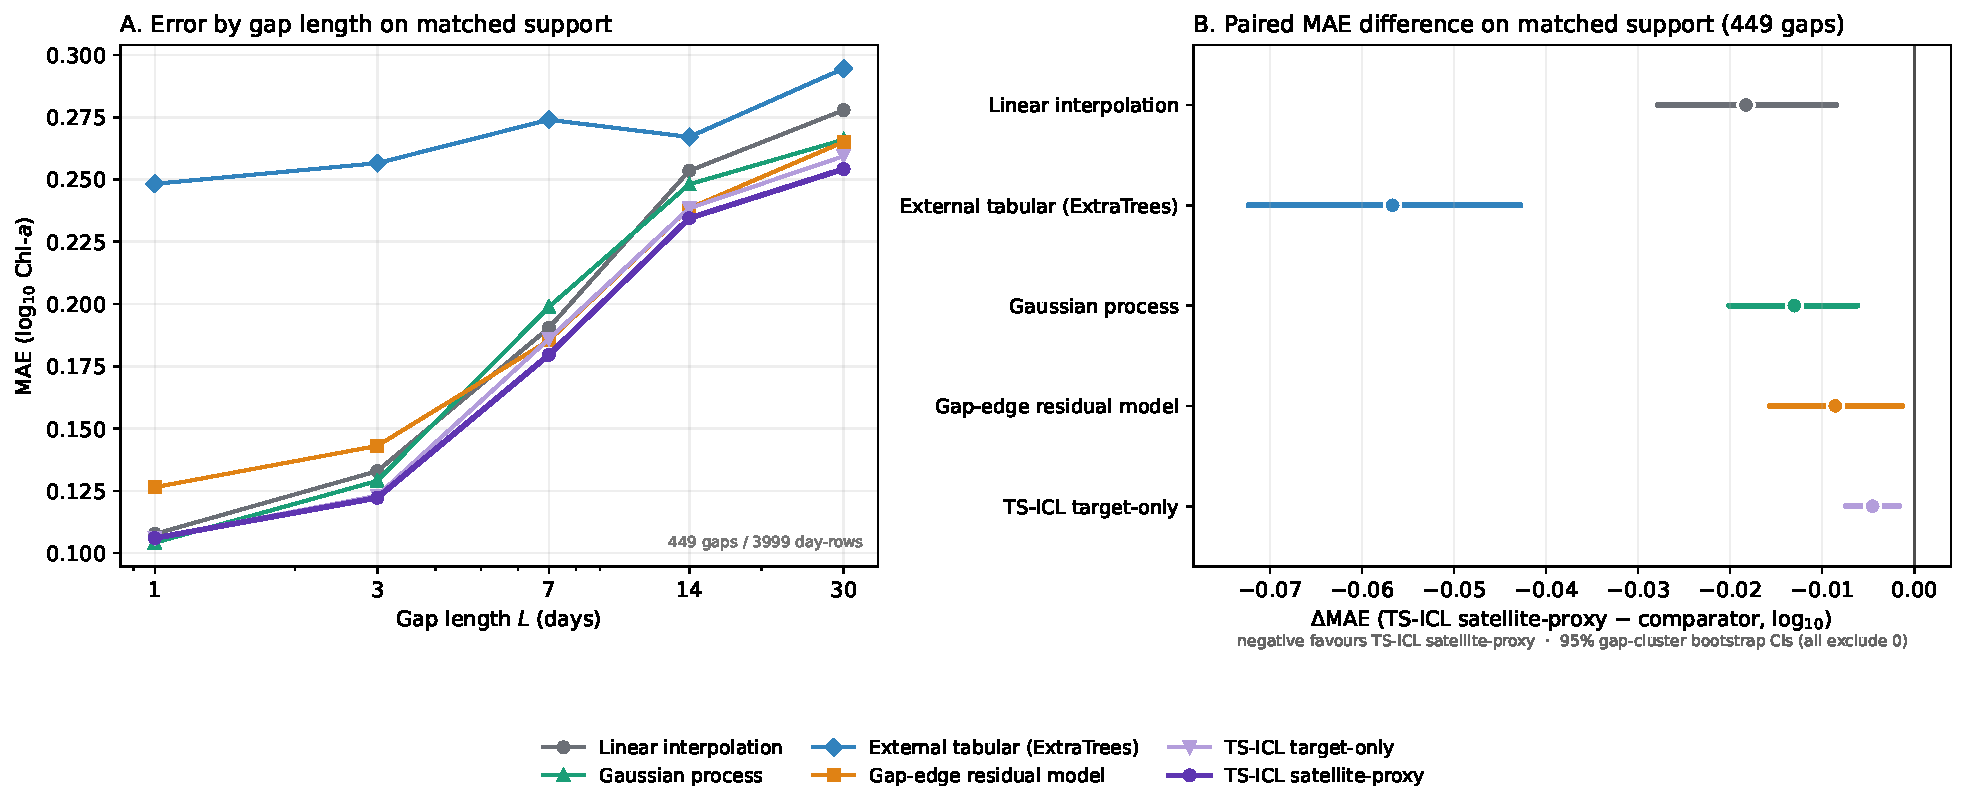
\includegraphics[width=\textwidth]{figures/fig4_chlorophyll_benchmark_matched.pdf}
  \caption{Artificial-gap chlorophyll benchmark.
  (A) Mean absolute error in $\log_{10}$ chlorophyll-\textit{a} by gap length. (B) Paired MAE difference
  between TS-ICL satellite-proxy and each comparator.}
  \label{fig:chl_benchmark_matched}
\end{figure}

TS-ICL also returns quantile predictions, here summarized by q05--q95 intervals. For the satellite-proxy
arm, empirical coverage is close to nominal at the three tested interval widths (Table~\ref{tab:tsicl_calibration}). This indicates that the reported uncertainty bands are generally informative, which matters here because real imputation scenarios have no withheld truth and should not be presented as point estimates alone.

\begin{table}[h]
  \centering
  \caption{TS-ICL satellite-proxy quantile calibration on the full 681-gap diagnostic pool.}
  \label{tab:tsicl_calibration}
  \begin{tabular}{rrr}
    \toprule
    Nominal interval & Empirical coverage & Difference \\
    \midrule
    50\% & 51.3\% & $+$1.3~pp \\
    80\% & 81.8\% & $+$1.8~pp \\
    90\% & 91.6\% & $+$1.6~pp \\
    \bottomrule
  \end{tabular}
\end{table}

\subsection{Covariate-signal checks}
\label{sec:chl_covariate_probe}

The TS-ICL covariate experiments provide a second way to test whether external predictors carry
usable reconstruction information. Unlike tabular feature importance, these checks do not depend
on a particular hand-engineered feature ranking. Each covariate
family is compared with placebo versions that preserve some marginal structure while breaking
the physically meaningful timing. Therefore a family is treated as carrying useful signal only
when the correctly aligned sequence beats the placebo alternatives with confidence intervals excluding zero.

Figure~\ref{fig:chl_covariate_placebo} shows the four-transform placebo battery for the physical
covariate families. Wind/upwelling forcing is the clearest physical signal: the aligned sequence
beats all four placebo variants. A curated physical-forcing set also survives the battery, but
with a smaller effect. Solar radiation gives mixed evidence, and SST/thermal forcing is not
robust under this criterion. Ocean current/transport covariates beat none of the placebo
variants, so the tested current inputs did not establish a usable chlorophyll reconstruction signal.

\begin{figure}[h]
  \centering
  \makebox[\textwidth][c]{%
    \hspace*{-1cm}%
    \resizebox{\textwidth}{!}{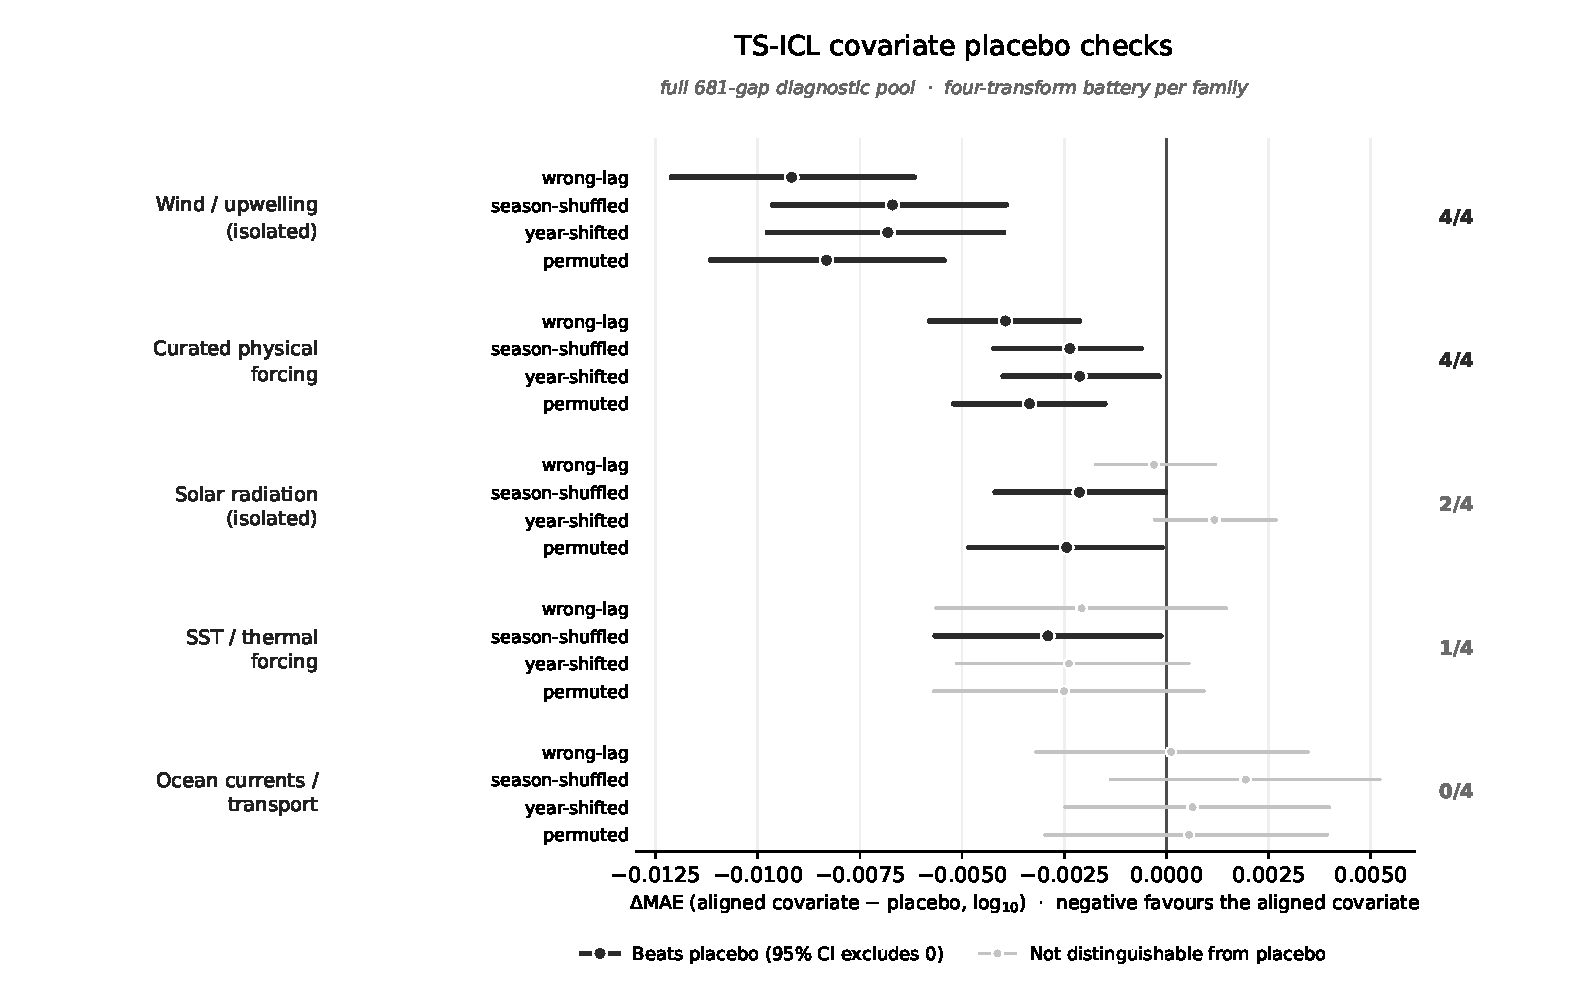
\includegraphics[width=0.92\textwidth]{figures/fig_chl_covariate_placebo_summary_v2.pdf}}%
  }
  \caption{TS-ICL covariate placebo checks for physical predictor families.
  Each row compares the correctly aligned covariate sequence with a disrupted placebo version. This is a full 681-gap TS-ICL diagnostic.}
  \label{fig:chl_covariate_placebo}
\end{figure}

\subsection{High-\texorpdfstring{\chl{}}{Chl-a} events remain difficult}
\label{sec:chl_events}

The benchmark identifies TS-ICL satellite-proxy as the strongest overall method, but the
event-stratified results show a clear limitation. All methods have higher MAE on high-\chl{}
event gaps than on non-event gaps (Figure~\ref{fig:chl_event_limitation}A). The external-only
tabular model is especially weak in this regime, consistent with the broader result that external
predictors alone do not reconstruct the target reliably. The gap-edge residual model and TS-ICL
reduce error relative to the weaker comparators, but neither removes the event penalty.

The illustrative artificial gap in Figure~\ref{fig:chl_event_limitation}B shows the nature of the
failure. The withheld event rises sharply inside the hidden interval. TS-ICL satellite-proxy has
the lowest error among the plotted methods for this gap, but its median reconstruction still
smooths and underestimates the event peak. Bloom events in this region can be short-lived and spatially patchy \citep{chavez2009comparison}, and all methods must infer the hidden event interior from boundary context, external covariates, or both.

\begin{figure}[h]
  \centering
  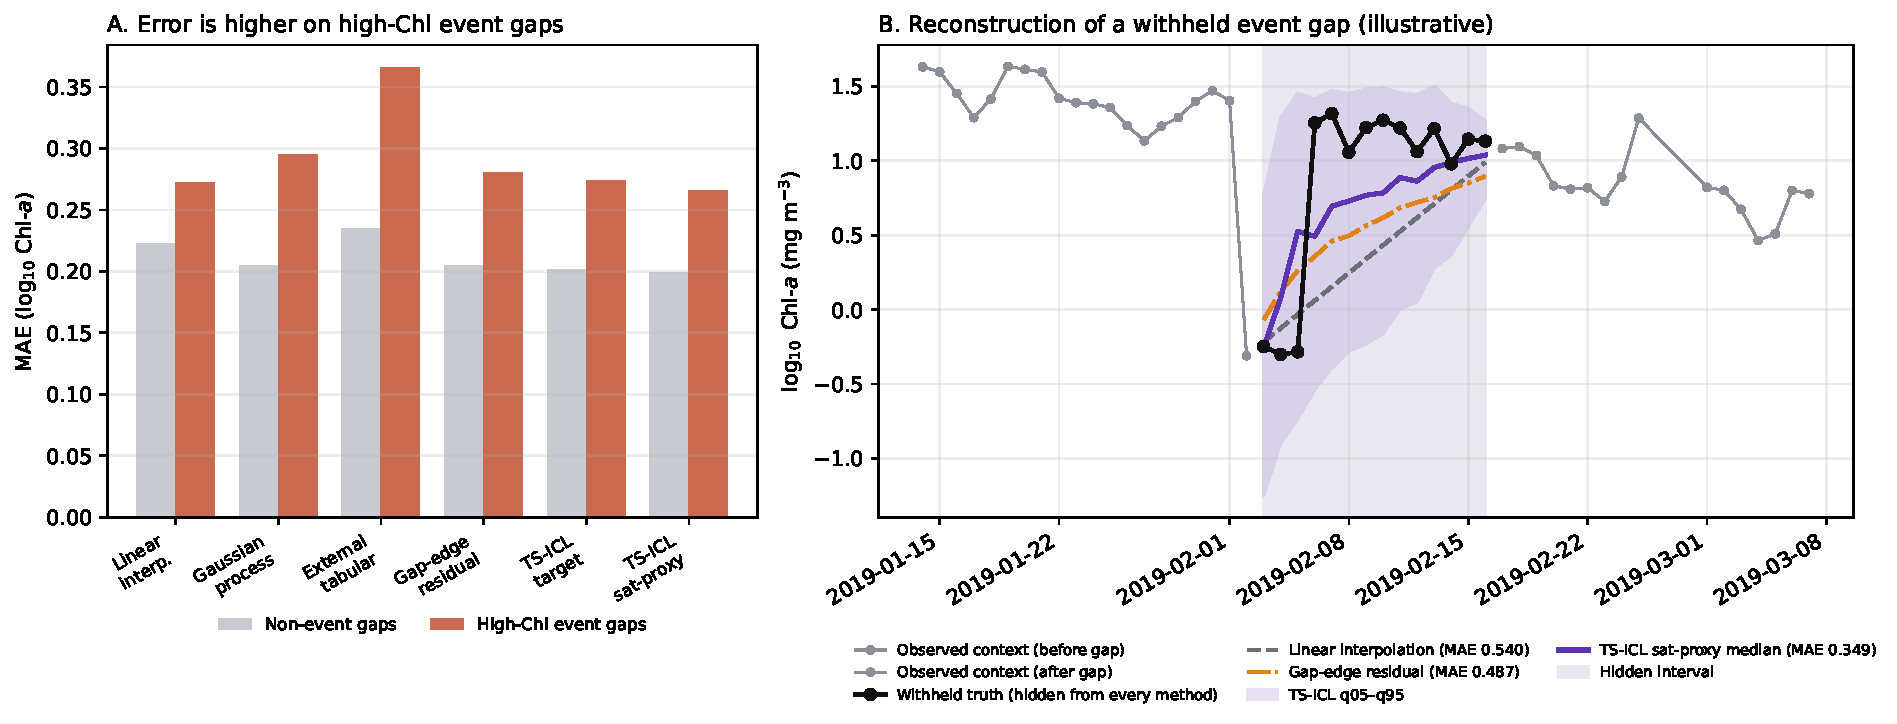
\includegraphics[width=\textwidth]{figures/fig5_event_limitation_matched_v2.pdf}
  \caption{High-\texorpdfstring{\chl{}}{Chl-a} event limitation.
  (A) Event and non-event MAE. All methods have higher error on
  high-\chl{} event gaps. (B) One withheld artificial 14-day event gap, shown as an illustrative
  example. Observed context is shown only outside the
  hidden interval; the black curve is the withheld truth used for artificial-gap scoring. For this
  example, per-gap MAE is 0.540 for linear interpolation, 0.487 for the gap-edge residual model,
  and 0.349 for TS-ICL satellite-proxy, but TS-ICL still underestimates the peak.}
  \label{fig:chl_event_limitation}
\end{figure}

\subsection{Real gaps: illustrative reconstructions, not validation}
\label{sec:chl_realgaps}

The benchmark evaluates reconstruction skill only on artificial gaps, where withheld
truth exists, while on real gaps the target was never observed, so no MAE or method ranking
can be computed. The TS-ICL satellite-proxy method was nevertheless applied to the real
chlorophyll gaps as an illustrative gap-filling output for practical use.

Figure~\ref{fig:chl_real_gap_multigap} shows one continuous 2015--2016 window containing six real
gaps of different lengths: 14, 15, 1, 1, 5, and 45 days.
All six gaps are within the artificial-gap validation range used in this report.
The main point is practical. TS-ICL can produce continuous candidate values across several real interruptions without fitting a separate station-specific model for each gap. The artificial-gap results above indicate how the method behaves when truth is available, while this figure shows how the selected method would be applied to actual missing intervals.

\begin{figure}[h]
  \centering
  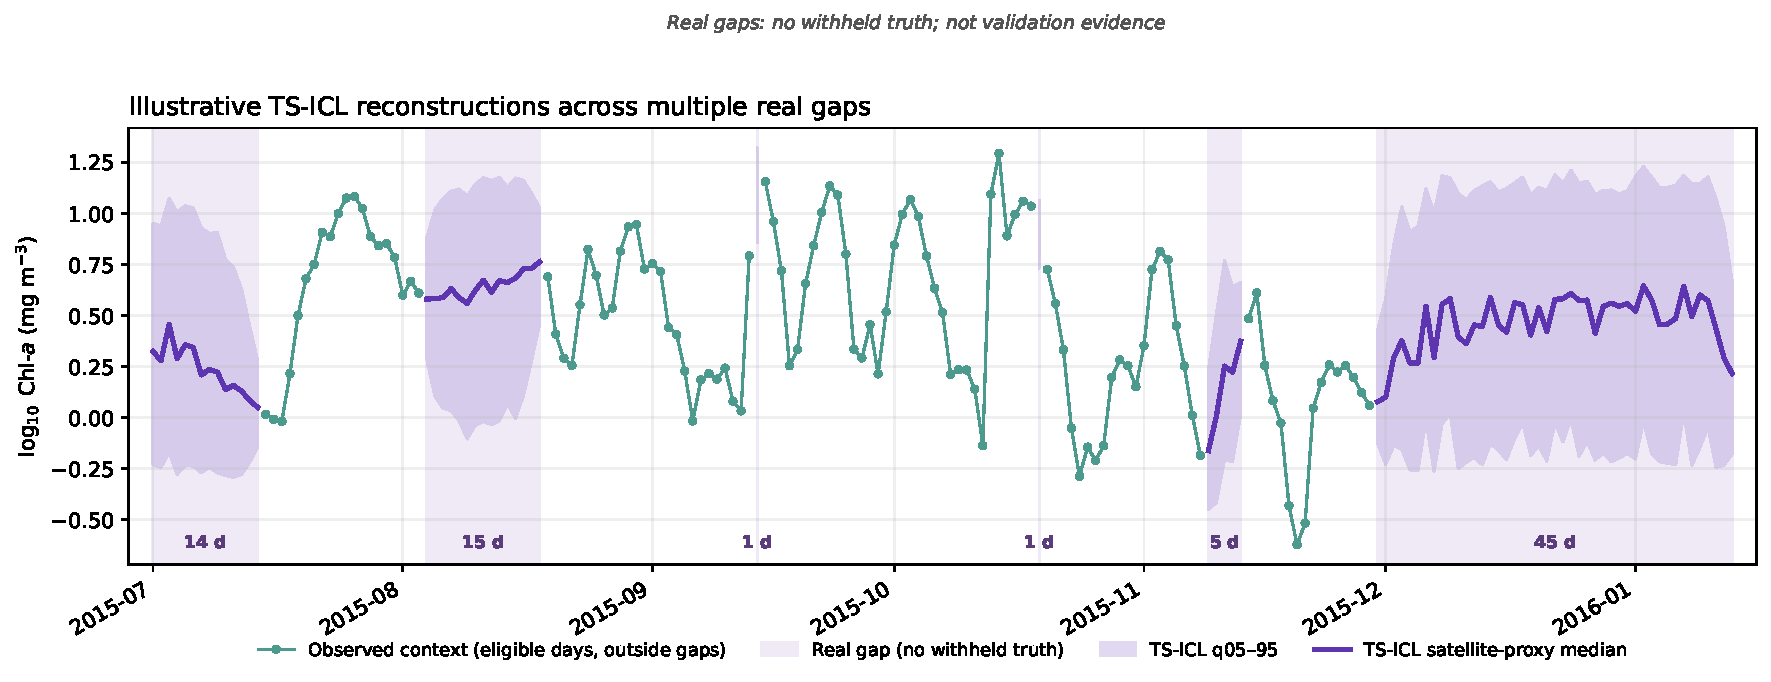
\includegraphics[width=0.95\textwidth]{figures/fig_chl_real_gap_multigap_v1.pdf}
  \caption{Illustrative chlorophyll real-gap reconstructions. A continuous 2015--2016 window is shown with six real gaps.}
  \label{fig:chl_real_gap_multigap}
\end{figure}

